%%%%%%%%%%%%%%%%%%%%%%%%%%%%%%%%%%%%%%%%
% Short Sectioned Assignment
% LaTeX Template
% Version 1.0 (5/5/12)
%
% This template has been downloaded from:
% http://www.LaTeXTemplates.com
%
% Original author:
% Frits Wenneker (http://www.howtotex.com)
%
% License:
% CC BY-NC-SA 3.0 (http://creativecommons.org/licenses/by-nc-sa/3.0/)
%
%%%%%%%%%%%%%%%%%%%%%%%%%%%%%%%%%%%%%%%%%

%----------------------------------------------------------------------------------------
%   PACKAGES AND OTHER DOCUMENT CONFIGURATIONS
%----------------------------------------------------------------------------------------

% A4 paper and 12pt font size separate paragraph
\documentclass[parskip=full, paper=a4, fontsize=12pt]{scrartcl} 

\usepackage[T1]{fontenc} 
\usepackage{fourier} 
\usepackage[english]{babel} 
\usepackage{amsmath,amsfonts,amsthm} 
\usepackage{color}
\usepackage{lipsum} 
\usepackage{hyperref}
\usepackage{subfigure}
\usepackage{sectsty} 
\usepackage{graphicx}
\usepackage{booktabs}
\usepackage[toc,page]{appendix}
\allsectionsfont{\normalfont\scshape} 

\usepackage{fancyhdr} 
\pagestyle{fancyplain} 
\fancyhead{} 
\fancyfoot[L]{} 
\fancyfoot[C]{} 
\fancyfoot[R]{\thepage} 
\renewcommand{\headrulewidth}{0pt} 
\renewcommand{\footrulewidth}{0pt} 
\setlength{\headheight}{13.6pt} 

\numberwithin{equation}{section} 
\numberwithin{figure}{section} 
\numberwithin{table}{section} 

\setlength\parindent{0pt} 

%-------------------------------------------------------------------------------
%	TITLE SECTION
%-------------------------------------------------------------------------------

\newcommand{\horrule}[1]{\rule{\linewidth}{#1}} 

\title{%	
\normalfont \normalsize 
\textsc{University of Crete\\
Computer Science Department \\
CS-446 -- Managed Runtime Systems} \\ [20pt] 
\horrule{0.5pt} \\[0.4cm]
\huge
Evaluating the Performance of Interpreters\\Over Various Branch Predictors
\horrule{2pt} \\[0.5cm] 
}

\author{%
    Emmanouil Pavlidakis \\
    Iacovos G. Kolokasis%
    } 

\date{\normalsize\today} 

\begin{document}

\maketitle 

%-------------------------------------------------------------------------------
%   INTRODUCTION	
%-------------------------------------------------------------------------------
\section{Introduction}

% What is an interpreter
Interpreters are widely used, since they provide portability on
different architectures, ease of implementation, and dynamic typing.
They transform a high-level programming language (source code), either
into machine code or into an intermediate language (i.e. byte code).
This byte code can be generated before actual execution(statically) as
in Java, or just before execution as in Python, or at runtime as in
JavaScript. The interpreter reads each line of high level or byte code
and then converts or executes it directly. 

The interpreter consists of an infinite loop, that fetches, decodes
and executes commands.  According to ~\cite{ertl2003structure}, this
dispatch loop create a large number of indirect branches. At that time
(i.e. 2000), branch predictors were not efficient in predicting
accurately this type of branches. Consequently, the performance of
interpreters were poor, due to the large mis-prediction rate of
indirect branches.  

%Problem statement
In this project we examine the performance of switch based
interpreters (Python, JavaScript, Java) on Intel and AMD
architectures. We focus on the impact of indirect branches, on state
of the art branch predictors, used by high end processors (Core2 duo,
Nehalem, Ivy Bridge, Haswell, AMD Bulldozer).

Our results show that mis-predictions for indirect branches, decreased
significantly from oldest to latest CPU generations (i.e. Core2 Duo to
Haswell). The average mis-predictions Per Kilo Instructions (MPKI) has
been decreased 2 times for Java, and almost 4 times for JavaScript and
Python, when comparing Core2 Duo and Haswell.   

%To be more specific, Python's Mis-predictions Per Kilo Instructions
%(MPKI) for all benchmarks is on average 0.7, while for Core2 Duo is
%2.7. In Java the average MPKI among all benchmarks is 8.9 for Haswell
%and for Core2 Duo is 19.4. Finally, in JavaScript the average MPKI is
%for Haswell 0.65, on the contrary for Core2 Duo is 2.9. As a result
%branch prediction is not an obstacle for interpreter's performance.

The rest of the report is organized as follows; section 2 describes the
experimental methodology.  Section 3 presents our results, while
sections 4 and 5 provide some conclusions and future work,
respectively.  

%-------------------------------------------------------------------------------
%   Experimental Methodology 
%-------------------------------------------------------------------------------
\section{Experimental Methodology}
% General description
This section describes the procedure that we follow, to collect the
mis-prediction data from indirect branches. Moreover, it describes the
hardware platforms and the interpreter versions and the benchmarks
that we use for our evaluation. 

% Interpreters and Benchmarks
\subsection{Interpreters}
We chose three switch based interpreted languages to evaluate; Python,
Java, and JavaScript. The selection of these particular languages
derive from GitHub results. According to
GitHub~\footnote{https://stackify.com/popular-programming-languages-2018/}
Python, Java and JavaScript are among the most popular runtime
languages. For Python we use the interpreter Pyhton3.6, for Java the
Java1.8.0, and for JavaScript Rhino 1.7R5. For Java and JavaScript we
disable JIT and all optimizations. 

\begin{table}[]
	\centering
	\caption{Interpreters and benchmark suites}
	\label{tab:inter_bench}
	\begin{tabular}{|c|c|c|}
		\hline
		\textbf{}           & \textbf{Interpreter} & \textbf{Suite}      \\ 
        \hline
		\textbf{Python}     & Python 3.6           & Python bench. suite \\ 
        \hline
		\textbf{Java}       & Java 1.8.0           & Dacapo-9.12         \\ 
        \hline
		\textbf{JavaScript} & Rhino 1.7R5          & Chrome octane 2.0   \\ 
        \hline
	\end{tabular}
\end{table}

\subsection{Benchmarks} 
To test Python's interpreter we run the Python Benchmark
suite~\footnote{https://github.com/python/performance}. For Java, we
utilize Dacapo-9.12 suite~\footnote{http://dacapobench.org/}, while
for for JavaScript we execute Chrome Octane 2.0
suite~\footnote{http://github.com/chromium/octane}.
Table~\ref{tab:inter_bench} displays an overall picture of the interpreter
versions and the benchmark suites used for the experiments.

Table~\ref{tab:benchmarks} lists all benchmarks for every suite. We
run each benchmark suite for 10 times. At every run we restart the
virtual machine. From Java and JavaScript suites we run all their
benchmarks (14, 13 respectively), on the contrary for Python we use
twenty benchmarks out of forty six. Ten out of forty six did not work,
from the remaining thirty six we exclude sixteen that do not have
different behavior from the reported ones.

\begin{table}
\centering
    \begin{tabular}{|l|l|l|}
        \hline
        \textbf{Python}         &\textbf{JavaScript}        &\textbf{Java} \\
        \hline
        bm\_2to3.py             &run\_box2d.js              &avrora     \\
        bm\_chaos.py            &run\_code\_load.js         &batik      \\
        bm\_deltablue.py        &run\_crypto.js             &eclipse    \\
        bm\_fankuch.py          &run\_deltablue.js          &fop        \\
        bm\_float.py            &run\_early\_boyer.js       &h2         \\
        bm\_go.py               &run\_gbemu.js              &jython     \\
        bm\_hexiom.py           &run\_navier-strokes.js     &luindex    \\
        bm\_json\_dumps.py      &run\_raytrace.js           &lusearch   \\
        bm\_json\_loads.py      &run\_regexp.js             &pmd        \\
        bm\_logging.py          &run\_richards.js           &sunflow    \\
        bm\_mdp.py              &run\_splay.js              &tradebeans \\
        bm\_meteor\_contest.py  &run\_typescript.js         &tradesoap  \\
        bm\_nbody.py            &run\_zlib.js               &xalan      \\
        bm\_nqueens.py          &                           &           \\
        bm\_pathlib.py          &                           &           \\
        bm\_piddigits.py        &                           &           \\
        bm\_pyflate.py          &                           &           \\
        bm\_python\_startup.py  &                           &           \\
        bm\_raytrace.py         &                           &           \\
        bm\_regex\_compile.py   &                           &           \\
        \hline
    \end{tabular}
    \caption{Benchmarks for JavaScript, Python and Java interpreters}
    \label{tab:benchmarks}
\end{table}
\subsection{Hardware platforms}
The evaluation of switch based interpreters, is performed on top of
actual (not emulated) branch predictors. We run our experiments to
Intel and AMD architectures, described in detail at Table~\ref{hw_p}.

\begin{table}[]
	\centering
	\caption{Hardware platforms}
	\label{hw_p}
	\begin{tabular}{|c|c|}
		\hline
		\textbf{}                           & \textbf{Description}                      \\ 
        \hline
		\textbf{Core 2 Duo (2006)}          & Intel Xeon(R) CPU E5405 at 2.00GHz        \\ 
        \hline
		\textbf{Nehalem (2008)}             & Intel Xeon(R) CPU E5520 at 2.27GHz        \\
        \hline
		\textbf{Ivy Bridge (2012)}          & Intel Xeon(R) CPU E5-2620 v2 at 2.10GHz   \\ 
        \hline
		\textbf{Haswell (2013)}             & Intel Xeon(R) CPU E5-2630 v3 at 2.40GHz   \\ 
        \hline
		\textbf{Buldoza family15th (2011)}  & AMD Opteron 6272 at 2.10GHz               \\ 
        \hline
	\end{tabular}
\end{table}

% Architectures
\subsection{Hardware Counters}
Hardware counters are collected by OProfile
1.2.0~\footnote{http://oprofile.sourceforge.net/news/}, an open source
statistical profiler for Linux systems. All architectures provide counters for
total instructions and mis-predicted indirect branches.These metrics should be
common to all architecture in order to be comparable. We collect the total
instructions executed, included retired (i.e. executed instructions not
speculative). Moreover, we  store the mis-predicted indirect branches that are
actually executed (i.e. retired).

We calculate the Miss Prediction Per Kilo Instructions (MPKI) rate, which is an
illustrative metric as described in~\cite{performance_of_interpreters}. It is
calculated by the following formula:
\begin{center}
   $ MPKI = \frac{Miss Indirect Brach Predictions * 1000}{Total Instructions} $
\end{center}

%-------------------------------------------------------------------------------
%   EXPERIMENTAL RESULTS
%-------------------------------------------------------------------------------
\section{Experimental Results}
%%%%%%%%%%%%%%%%%%%%%%%%%%%%%%%  PYTHON   %%%%%%%%%%%%%%%%%%%%%%%%%%%%%%%%%%%
\subsection{Python}
\begin{figure*}[t]
	\centering
	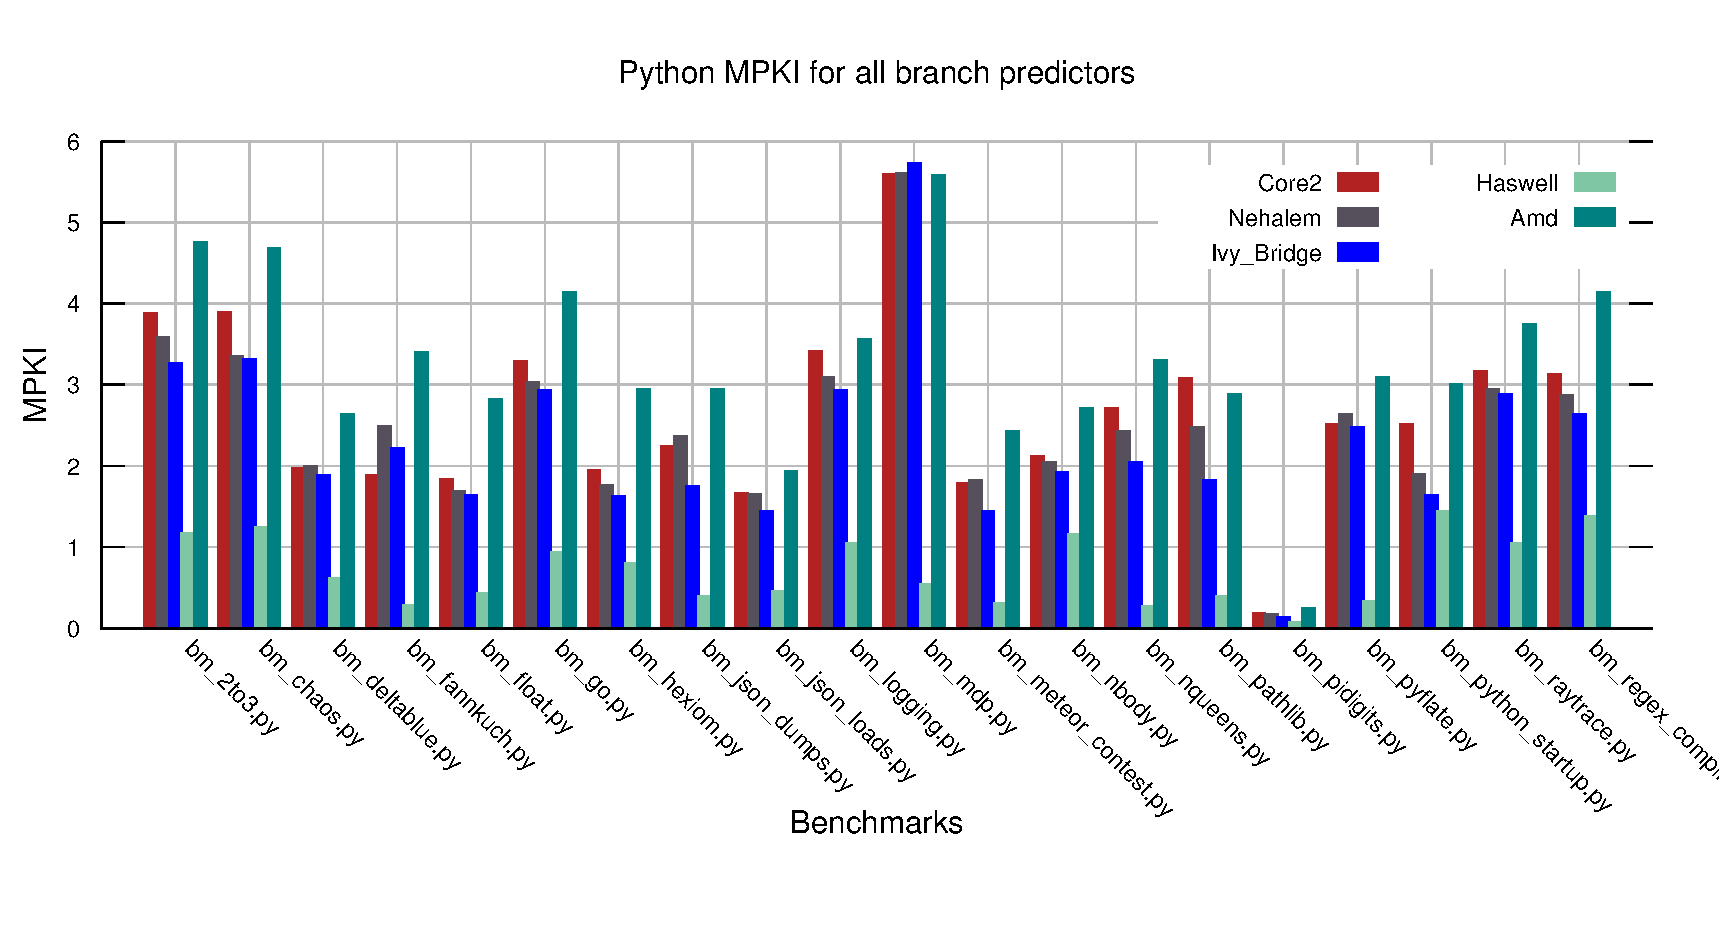
\includegraphics[width=1\textwidth]{figures/python_MPKI.pdf}
	\caption{MPKI for Python 3.6 over all architectures}
	\label{fig:pythonmpki}
\end{figure*}
Figure~\ref{fig:pythonmpki} describes MPKI for Python language, with the interpreter python3.6 for all architectures. As we can observe Haswell has the lowest mis-prediction rate (on average 0.7), while AMD family15th the highest (on average 2.7). If we focus only in Core 2, Nehalem, and Ivy Bridge, as the CPU's generation increases the MPKI decreases. However, in some benchmarks such as \textit{json loads}, \textit{mdp}, \textit{meteor contest}, and \textit{pyflate} as Core2 has better performance Nehalem. This happens because some generations probably have optimizations for specific cases which are not included from others.  

Figure (Appendices)~\ref{res:pythonbox} shows the MPKI variation, of ten iterations, per benchmark. We can observe that there is no significant variation among iterations.

%%%%%%%%%%%%%%%%%%%%%%%%%%%%%%%  JAVA   %%%%%%%%%%%%%%%%%%%%%%%%%%%%%%%%%%%
\subsection{Java}

\begin{figure*}[t]
	\centering
	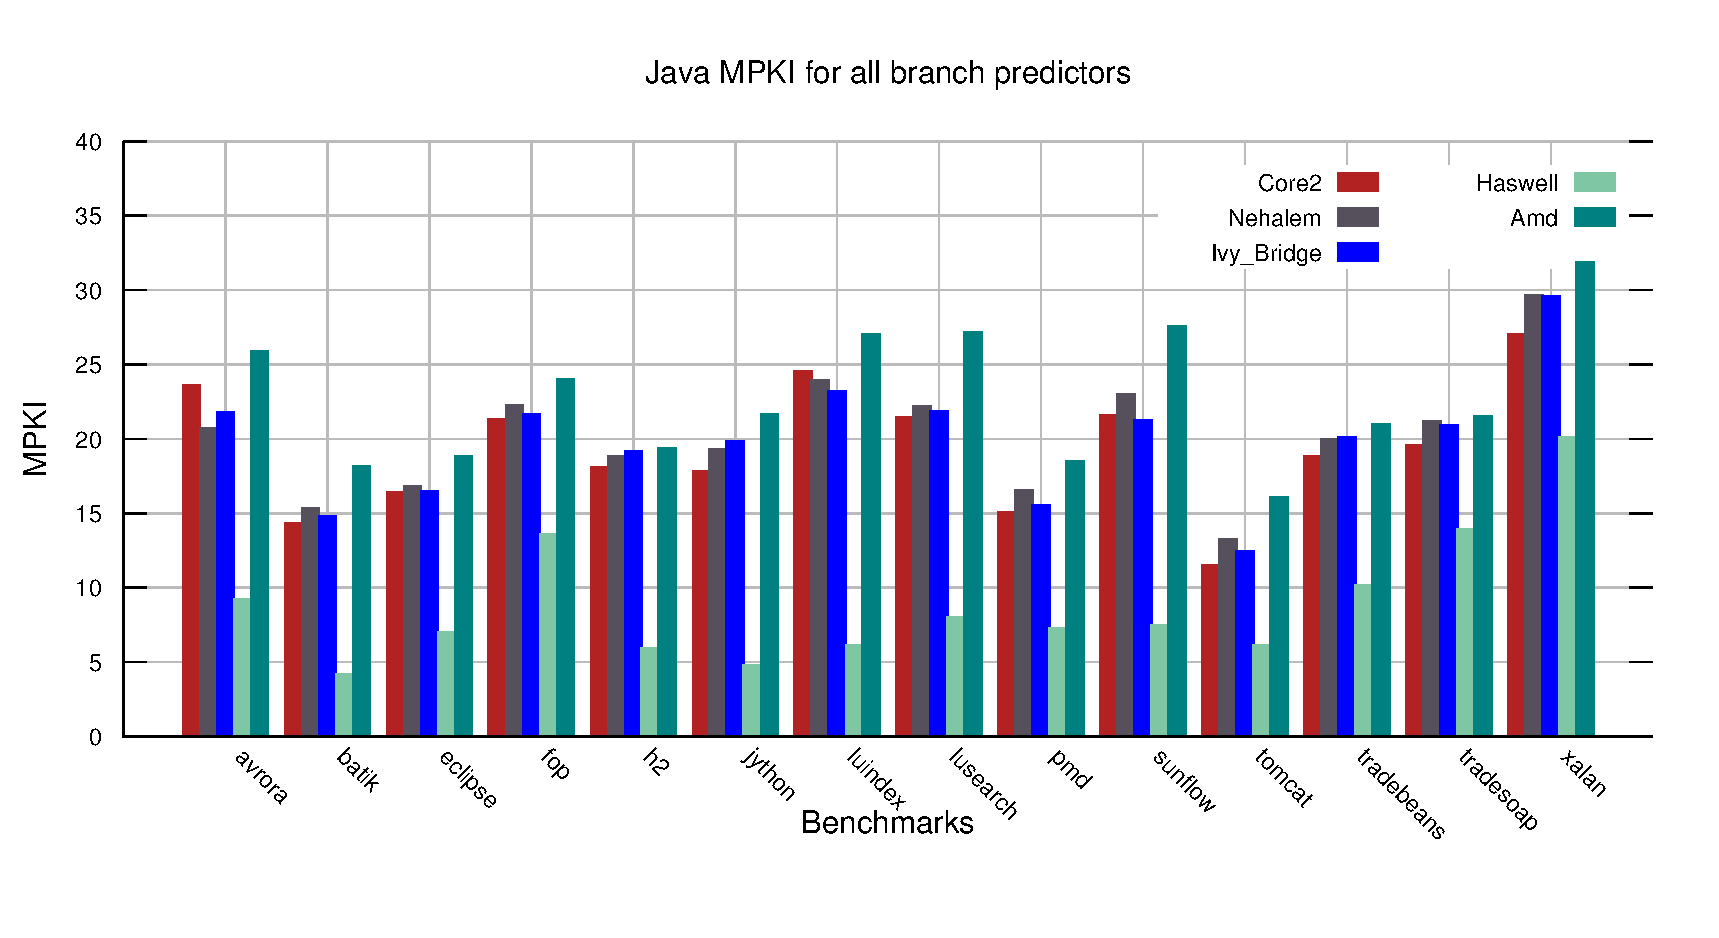
\includegraphics[width=1\textwidth]{figures/java_MPKI.pdf}
	\caption{MPKI for Java 1.8.0 over all architectures}
	\label{fig:javampki}
\end{figure*}

Figure~\ref{fig:javampki} describes MPKI for Java language, with the interpreter java 1.8.0 among all architectures. As in Python, Haswell has again the lowest mis-prediction rate (on average 8.9), and AMD family15th the highest (on average 19.4) in all benchmarks. If we focus only in Core 2, Nehalem, and Ivy Bridge, as the generation increases, the mis-prediction rate does not decrease in the majority of benchmarks. 

Figure (Appendices)~\ref{res:javabox} shows the MPKI variation, of ten iterations, per benchmark. We can observe that there is no significant variation among iterations.

%%%%%%%%%%%%%%%%%%%%%%%%%%%%%  JAVASCRIPT   %%%%%%%%%%%%%%%%%%%%%%%%%%%%%%%%
\subsection{JavaScript}

\begin{figure*}[t]
	\centering
	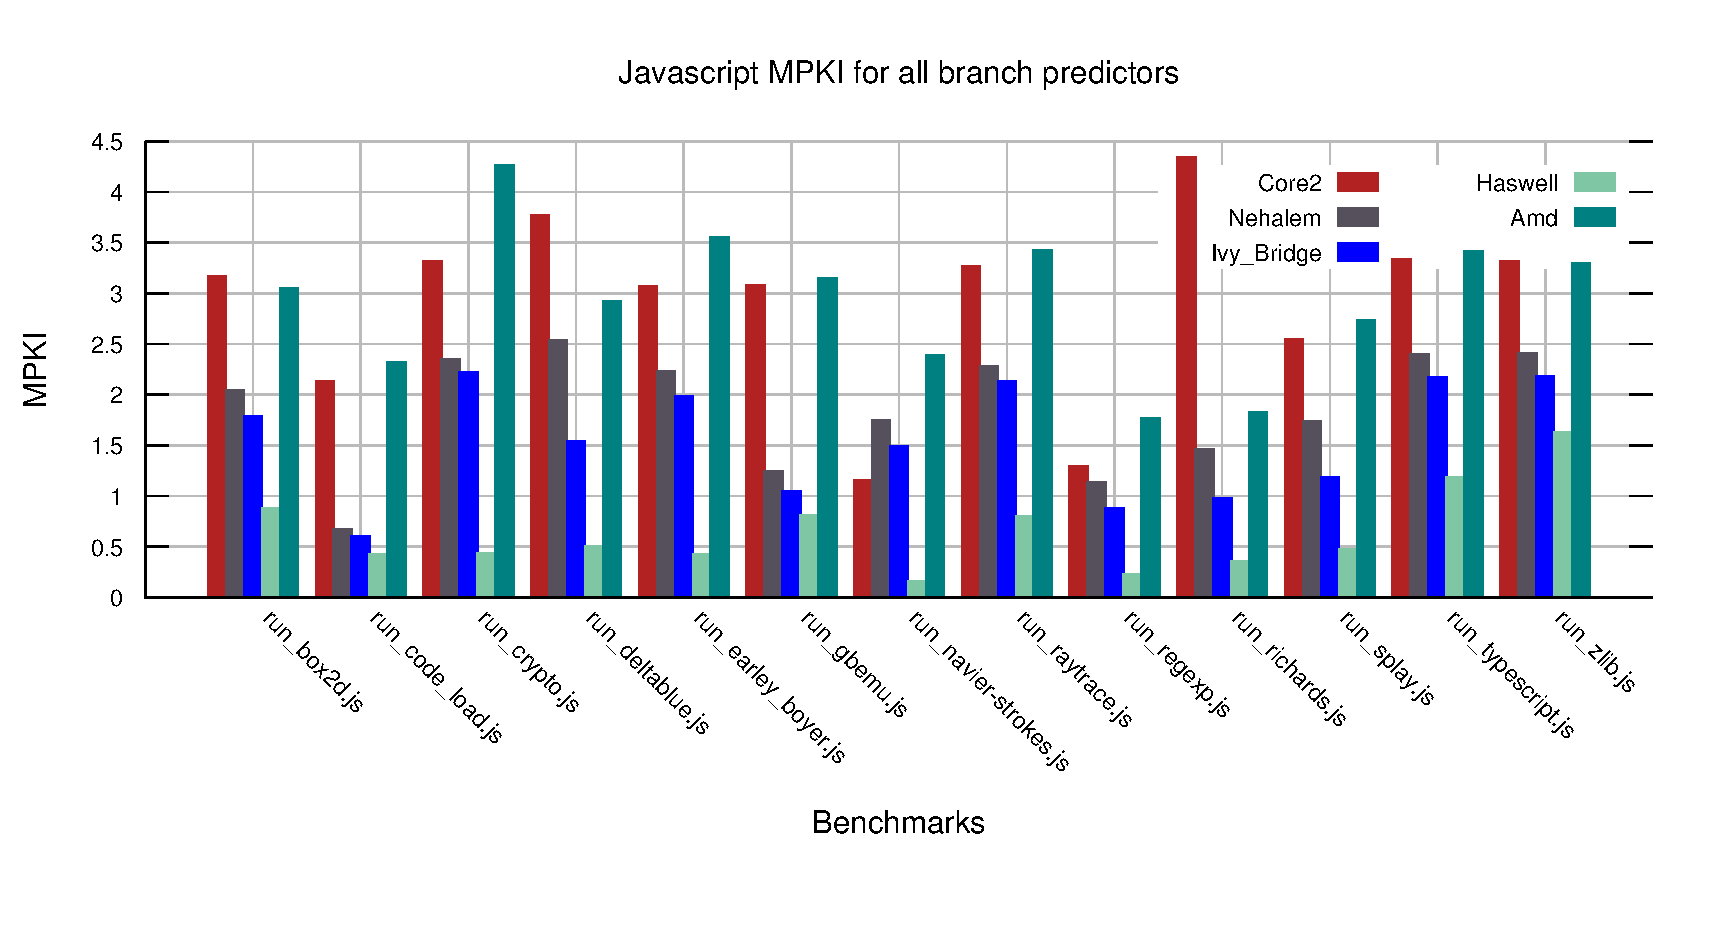
\includegraphics[width=1\textwidth]{figures/javascript_MPKI.pdf}
	\caption{Mis-predictions Per Kilo Instructions for Javascript (Rhino 1.7R5) over all architectures}
	\label{fig:javascriptmpki}
\end{figure*}
Figure~\ref{fig:javascriptmpki} describes MPKI for Javascript language, with the interpreter Rhino1.7R5. It has the same behavior as Python Figure~\ref{fig:pythonmpki}. Again Haswell has the lowest mis-prediction rate (on average 0.65), while AMD family15th the highest (on average 2.9). For all benchmarks as the generation increases the MPKI decreases significantly.  

Figure (Appendices)~\ref{res:pythonbox} shows the MPKI variation, of ten iterations, per benchmark. We can observe that there is variation for splay and delta blue in all architectures. The lowest variation is in Haswell (0.2 up to 0.8). This behavior derives from the implementation of that particular benchmark.    


%-------------------------------------------------------------------------------
%   CONCLUSIONS
%-------------------------------------------------------------------------------
\section{Conclusions}
Interpreted languages are very important and useful, because they provide platform independence, dynamic typing and ease of debugging. Due to their implementation they produce a huge number of indirect branches~\cite{performance_of_interpreters}. At 2000 branch predictors were not accurate in predicting this type of branches, consequently interpreter's performance was poor~\cite{performance_of_interpreters}. 

In this work we investigate how the mis-prediction rate, behaves across different CPU generations (i.e. different branch prediction policies) and if their accuracy in indirect branches has been improved. We show that in general as the generation increases the branch prediction rate for indirect branches decreases, sharply. The mis-predictions of Haswell, which is the newest generation that we evaluate, proves that indirect branches are not a performance obstacle for interpreters anymore. As displayed in Table~\ref{mpkiimprovement} the mis-prediction rate has been improved up to 4 times, when comparing Core 2 Duo (oldest generation) and Haswell (newest generation).    

\begin{table}[]
	\centering
		\begin{tabular}{@{}|c|c|c|@{}}
			\toprule
			\textbf{}           & \textbf{Core2 Duo} & \textbf{Haswell} \\ \midrule
			\textbf{Python}     & 2.7                & 0.7              \\ \midrule
			\textbf{Java}       & 19.4               & 8.9              \\ \midrule
			\textbf{Javascript} & 2.9                & 0.65             \\ \bottomrule
		\end{tabular}
	\caption{AVG MPKI improvement from oldest to newest generation}
	\label{mpkiimprovement}
\end{table}
%-------------------------------------------------------------------------------
%   Future Work
%-------------------------------------------------------------------------------
\section{Future Work}
We plan to execute more experiments to evaluate extensively our findings.
Firstly we need to find the mis-predictions created from VMs. VM's code created mis-predictions at the start and at the end of the
VM execution. We have to isolate these mis-prediction created by
VMs. Then interpreter's mis-predictions rate will be more
accurate and will focus only to the indirect branches created by interpreters. 

It will be interesting to study different versions of interpreters, for instance Python2.7 versus Python3.6, or Rhino versus Spider Monkey. This will provide more details about the overhead created from interpreters and if their code has been improved. With this type of experiment, we will be able to determine
if the performance improvement of interpreters, is correlated with improvements in interpreters code or with modifications in the branch prediction policy of CPUs.  

\newpage
\bibliographystyle{abbrv}
\bibliography{cs446_Report}
\begin{appendices}
	\begin{figure*}[t]
		\subfigure[Core 2 Duo]
		{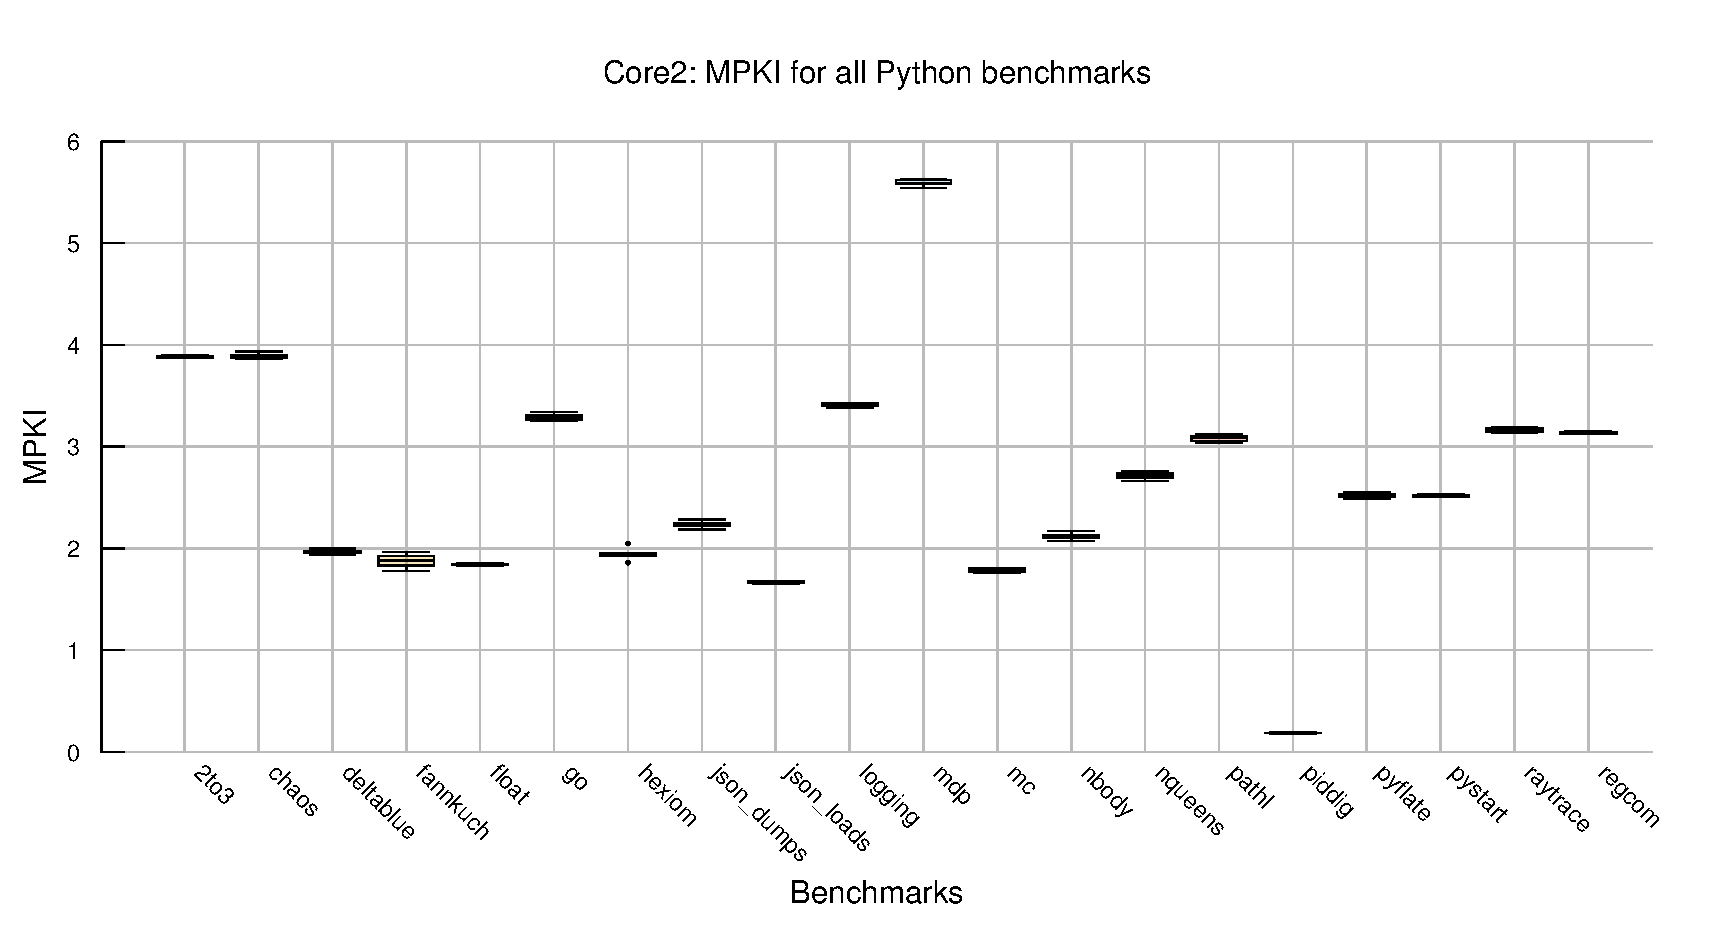
\includegraphics[width=0.5\textwidth]{figures/python_box_core2.pdf}}
		\subfigure[Nehalem]%
		{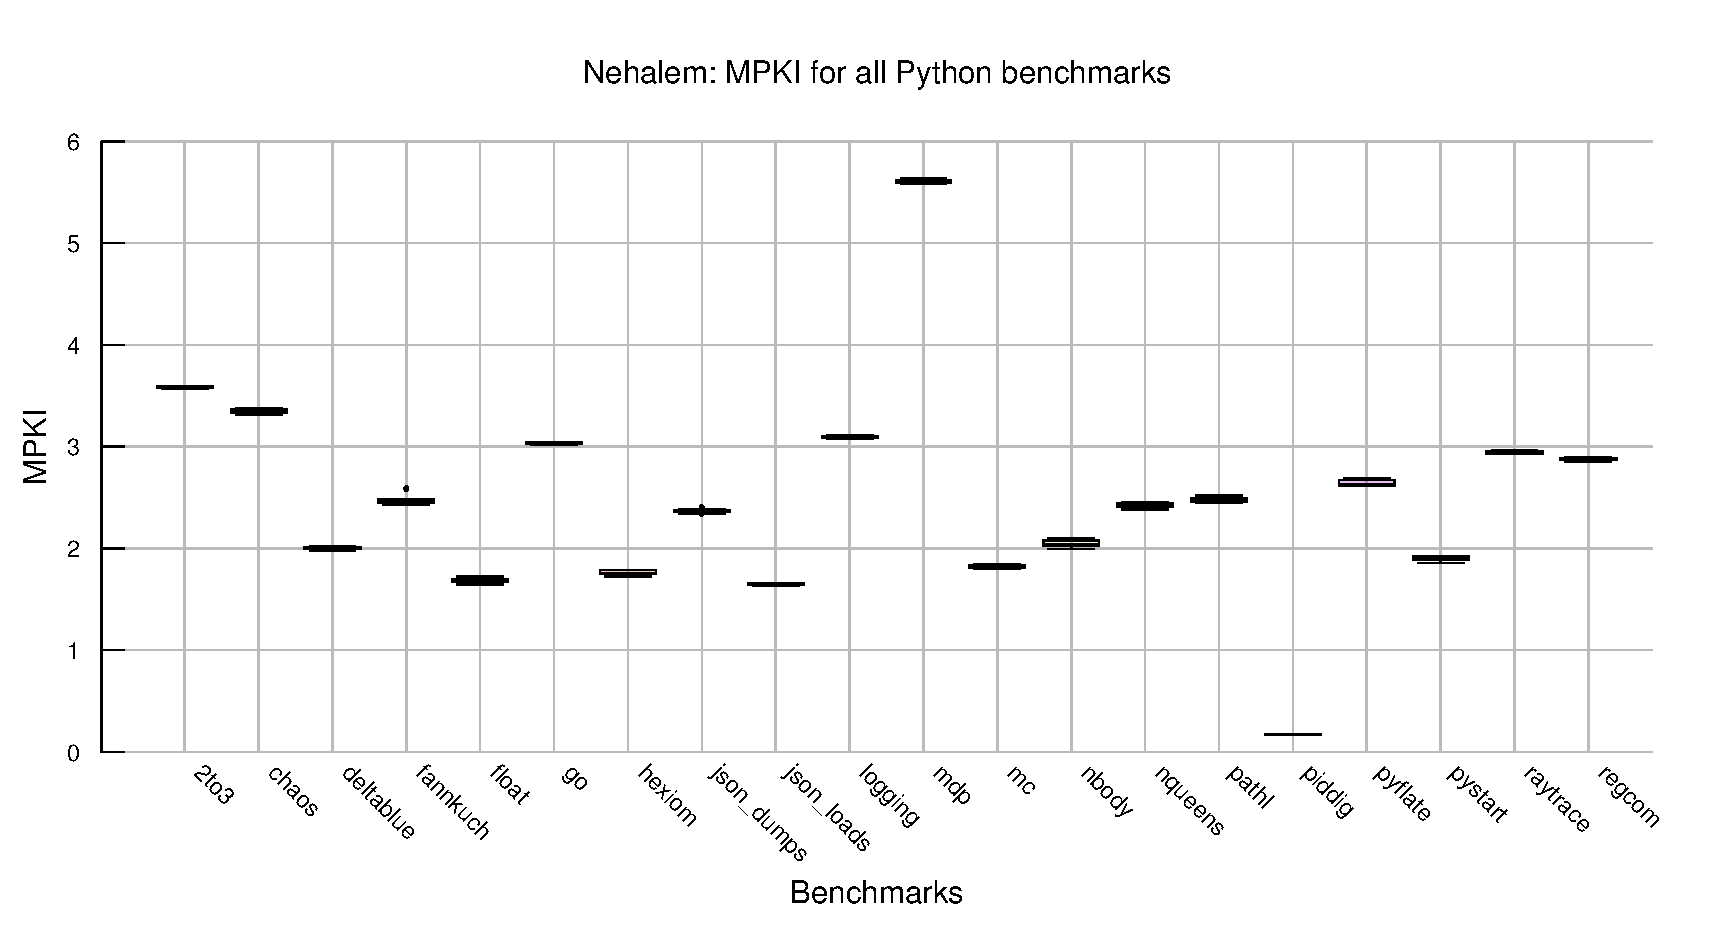
\includegraphics[width=0.5\textwidth]{figures/python_box_nehalem.pdf}}
		\subfigure[Ivy Bridge]
		{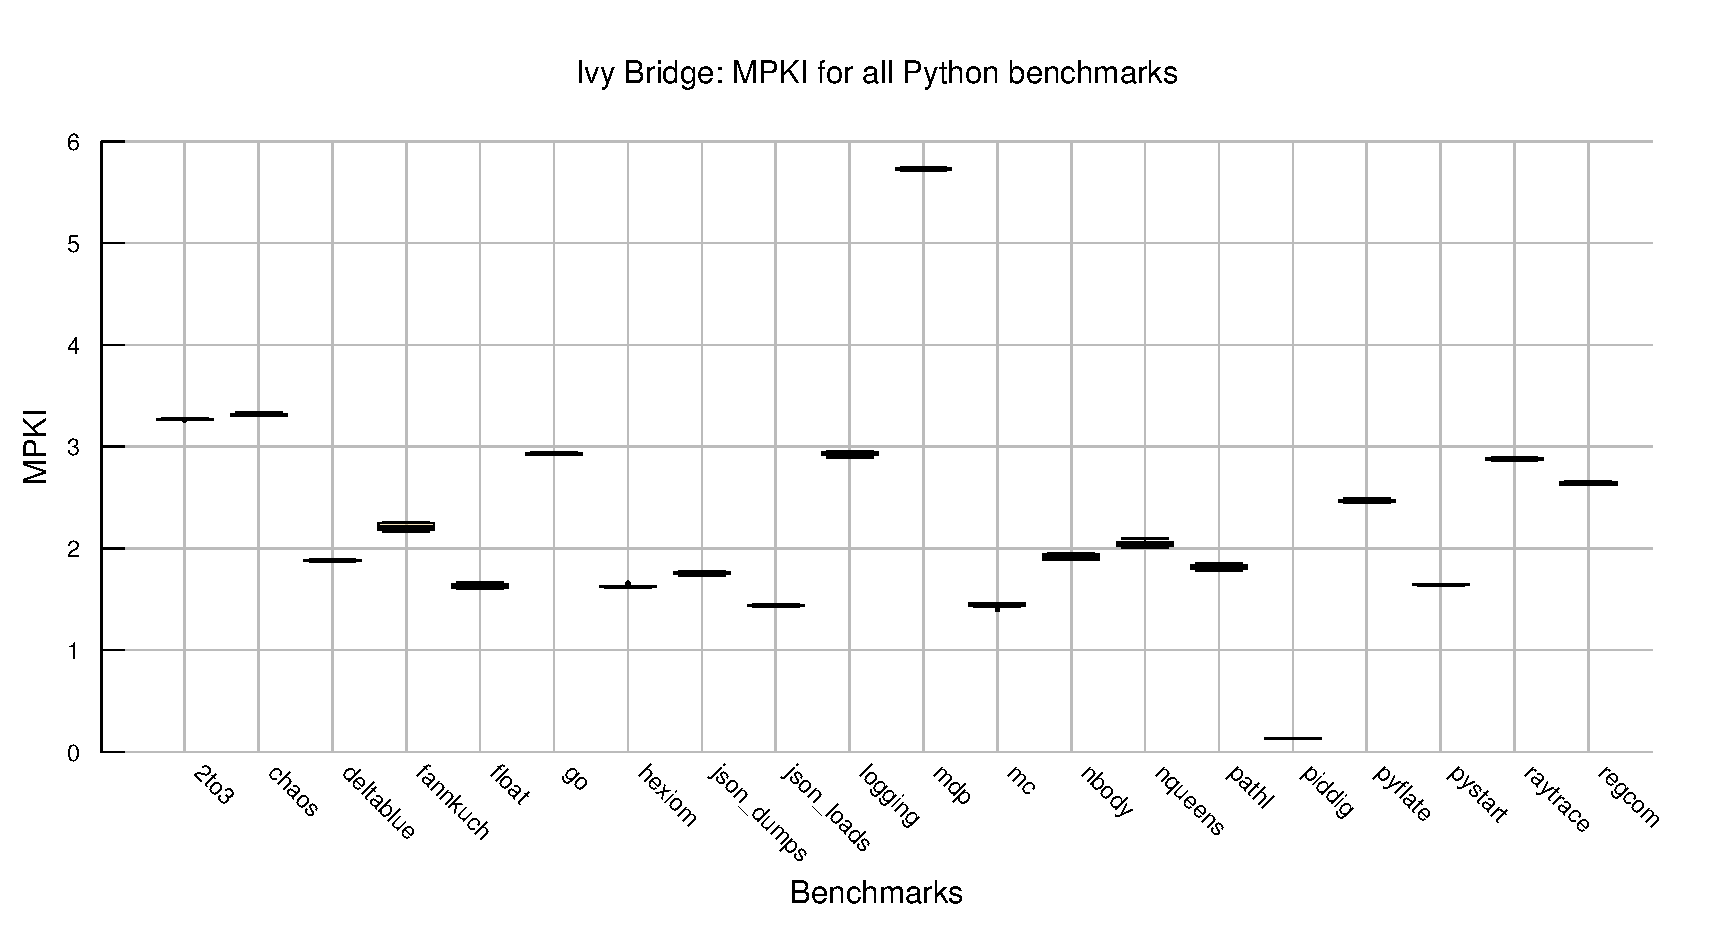
\includegraphics[width=0.5\textwidth]{figures/python_box_ivy_bridge.pdf}}
		\subfigure[Haswell]
		{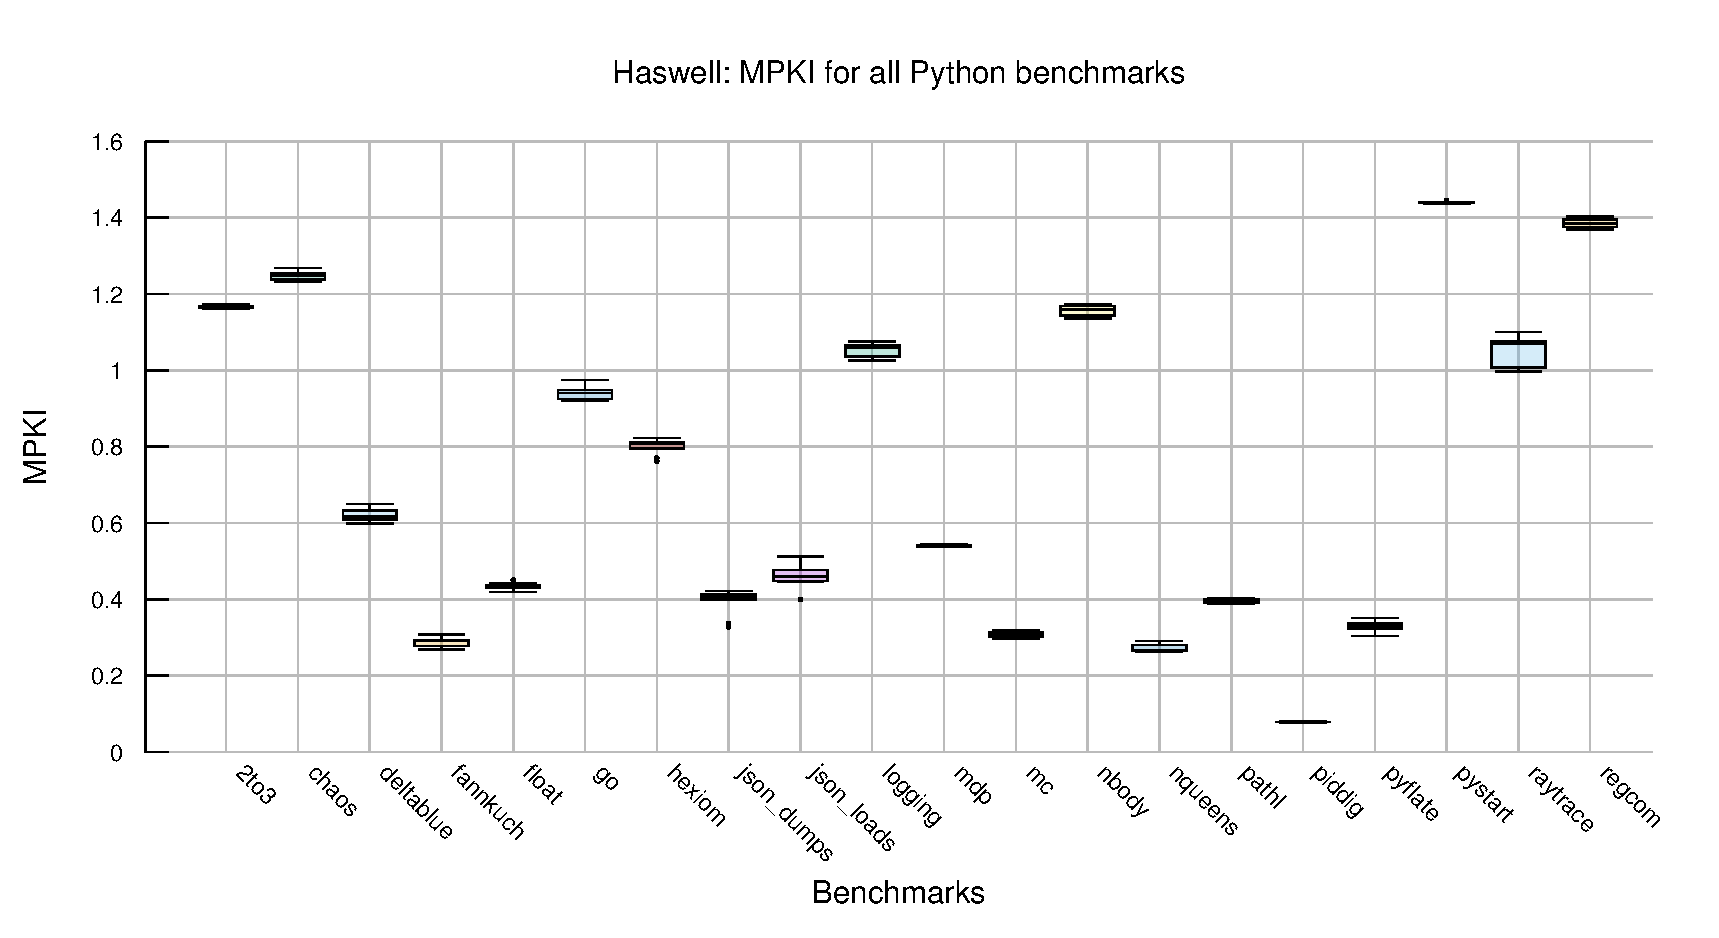
\includegraphics[width=0.5\textwidth]{figures/python_box_haswell.pdf}}
		\subfigure[AMD family15th]
		{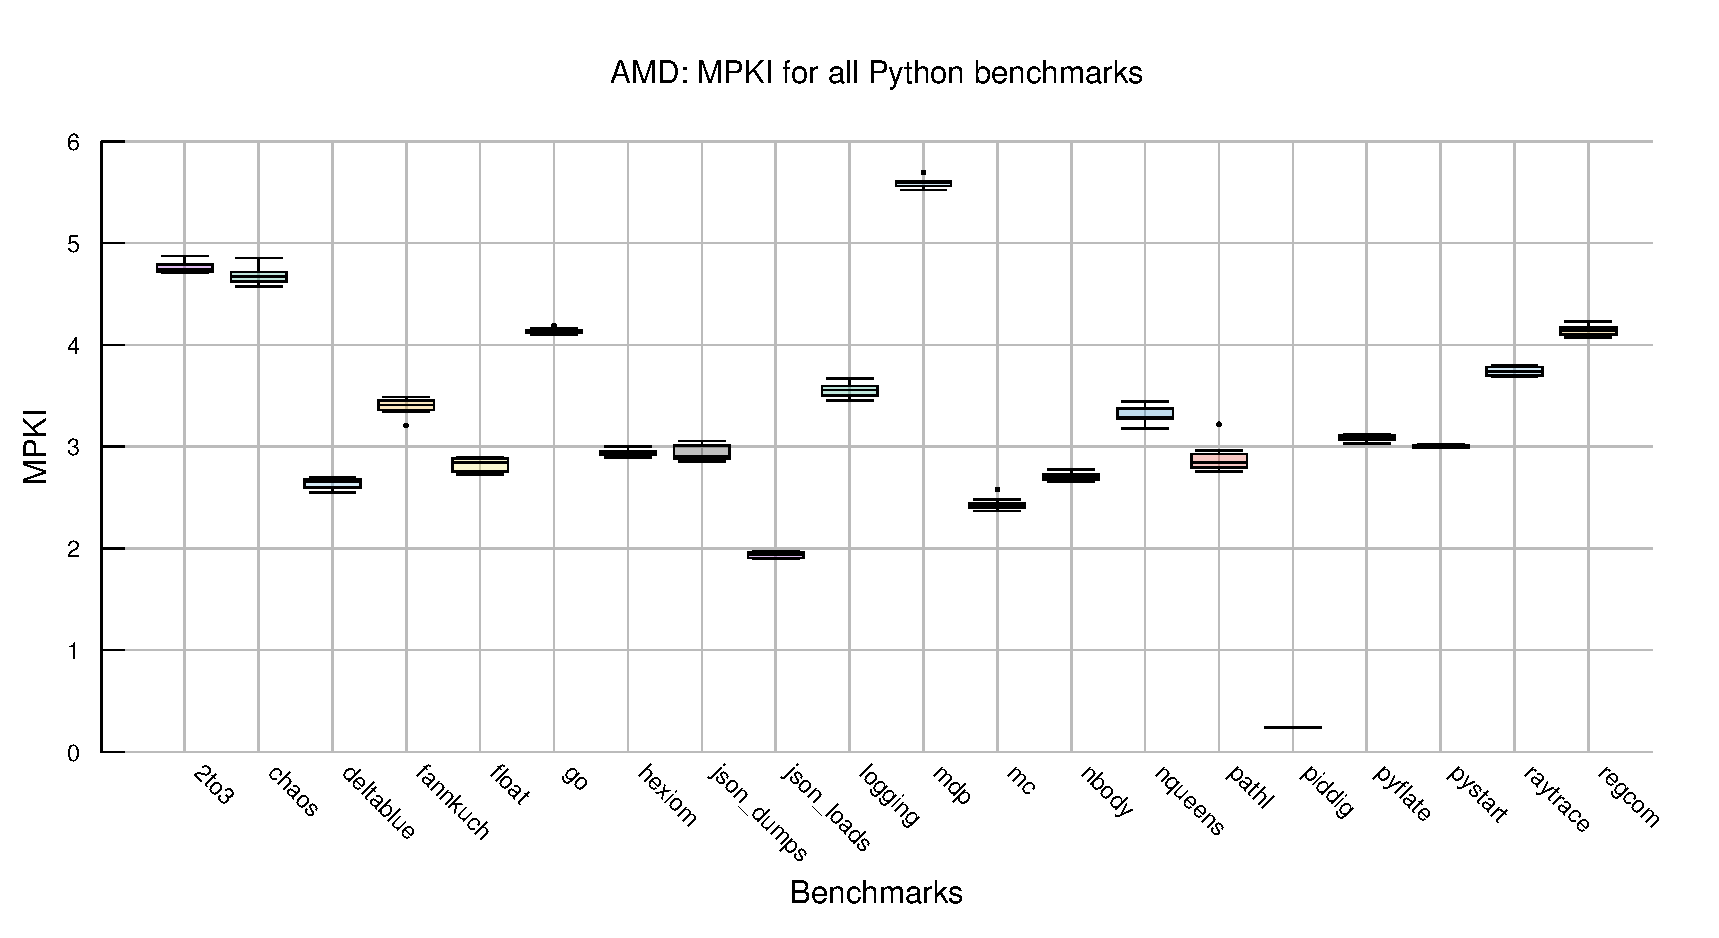
\includegraphics[width=0.5\textwidth]{figures/python_box_amd.pdf}}
		
		\caption{Python: Variation of MPKI for 10 iterations per benchmark for all architectures}
		\label{res:pythonbox}
	\end{figure*}
	\begin{figure*}[t]
		\subfigure[Core 2 Duo]
		{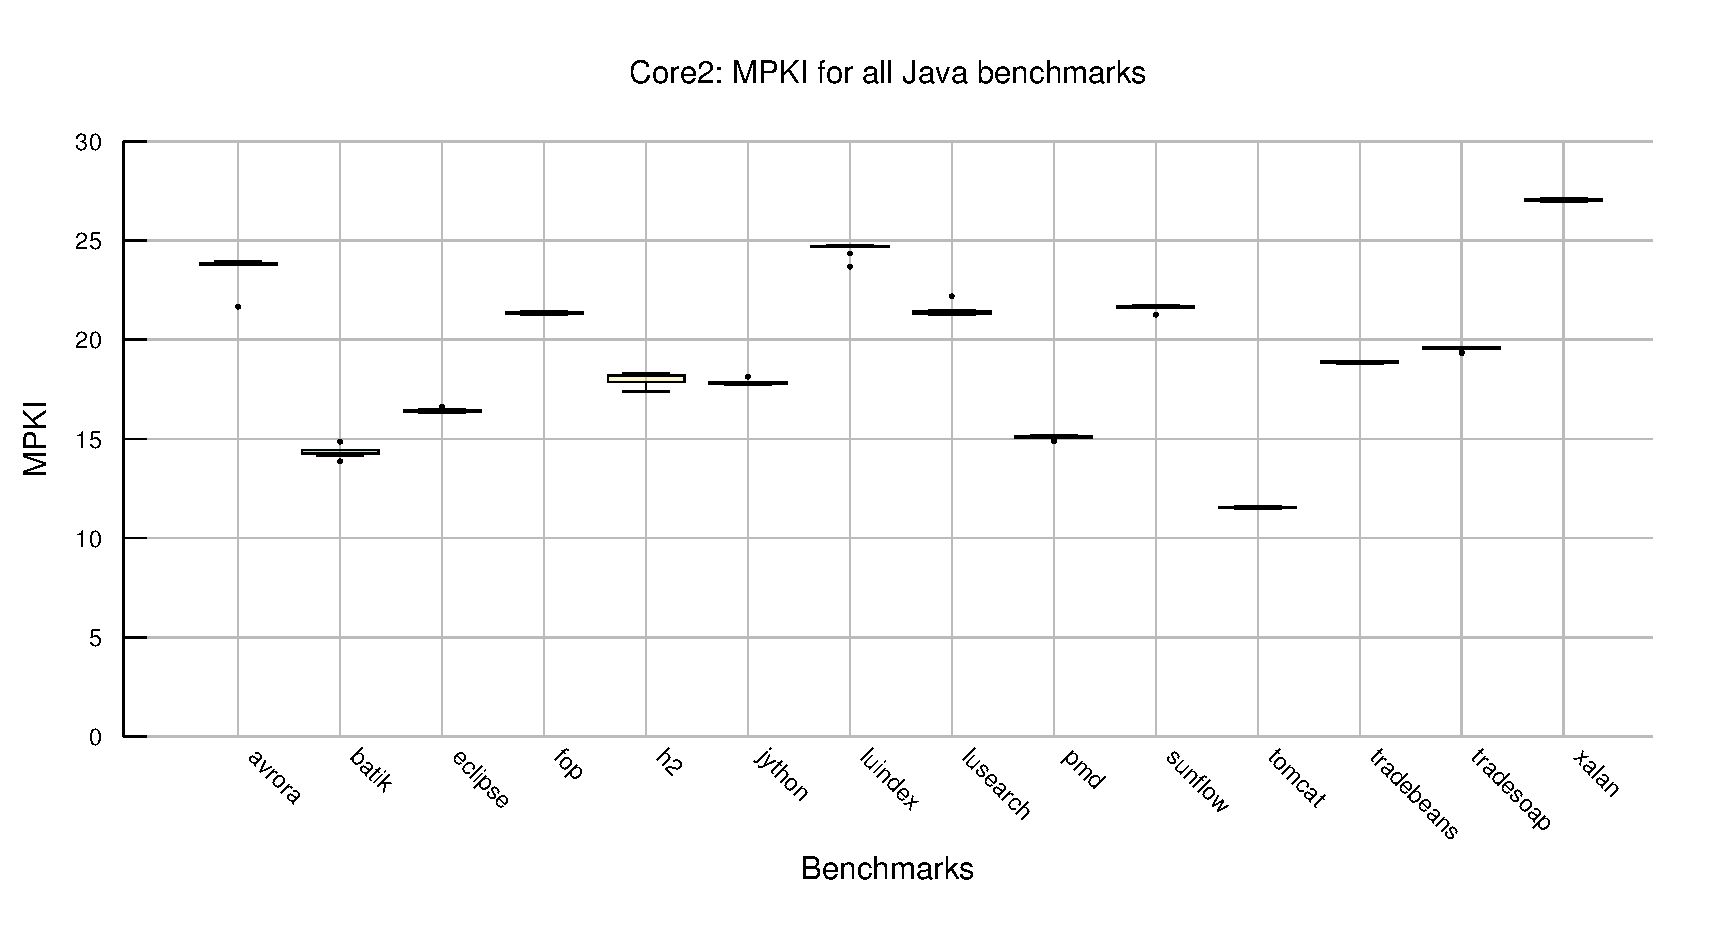
\includegraphics[width=0.5\textwidth]{figures/java_box_core2.pdf}}
		\subfigure[Nehalem]%
		{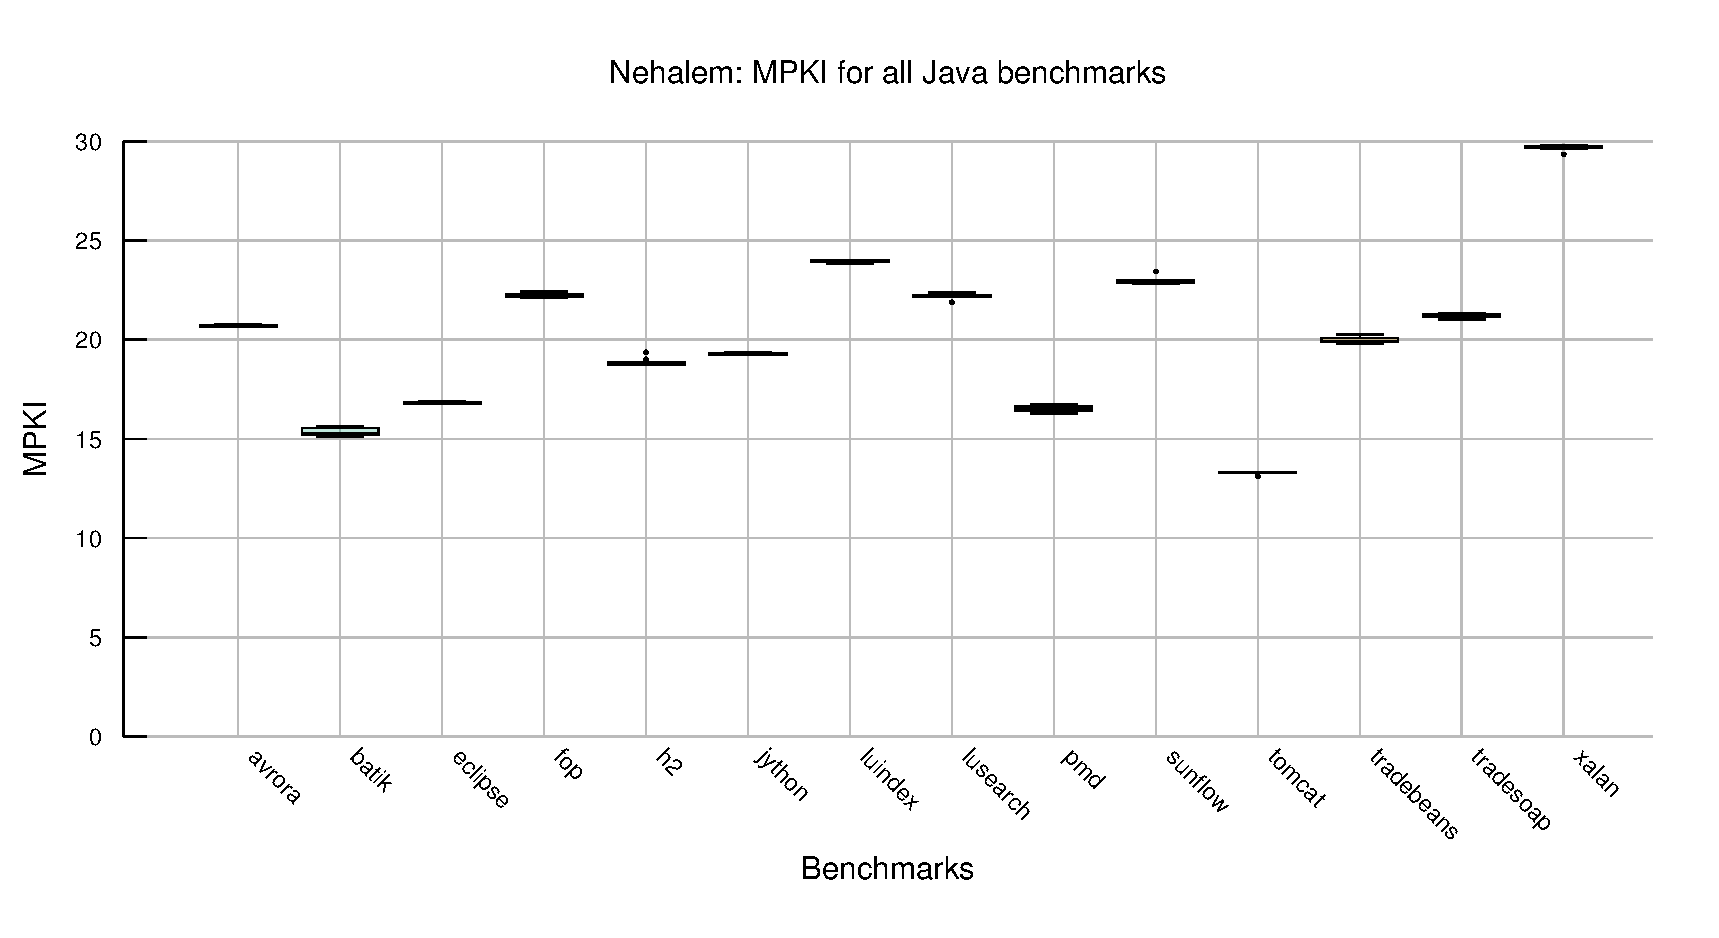
\includegraphics[width=0.5\textwidth]{figures/java_box_nehalem.pdf}}
		\subfigure[Ivy Bridge]
		{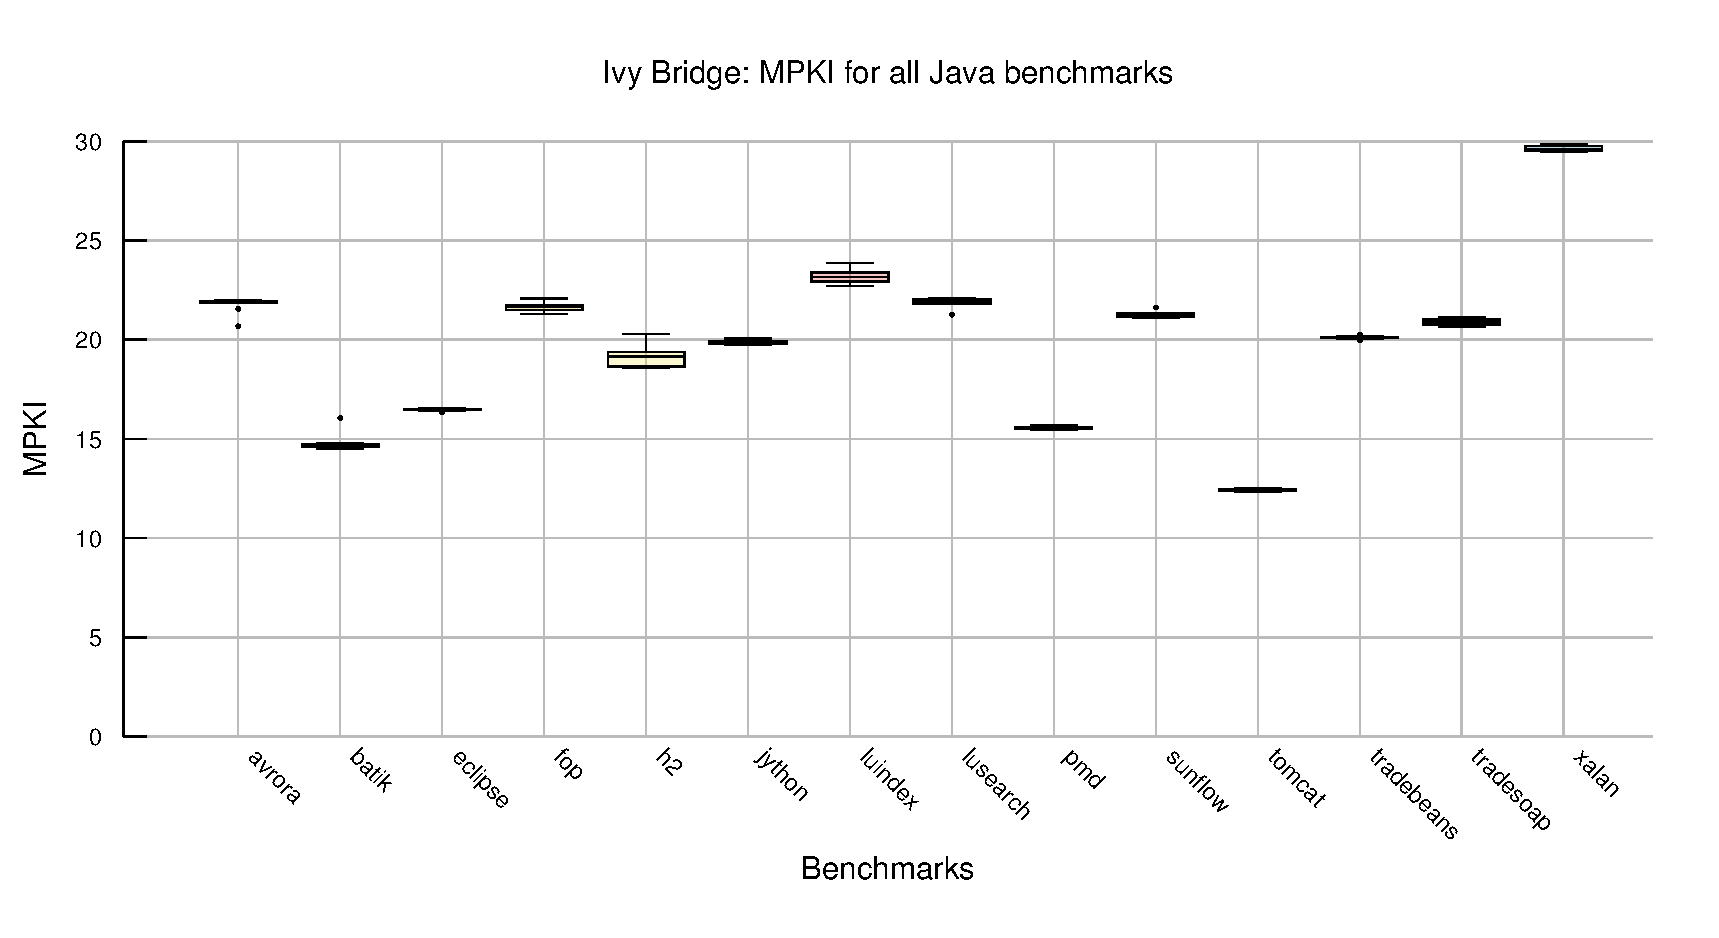
\includegraphics[width=0.5\textwidth]{figures/java_box_ivy_bridge.pdf}}	\subfigure[Haswell]
		{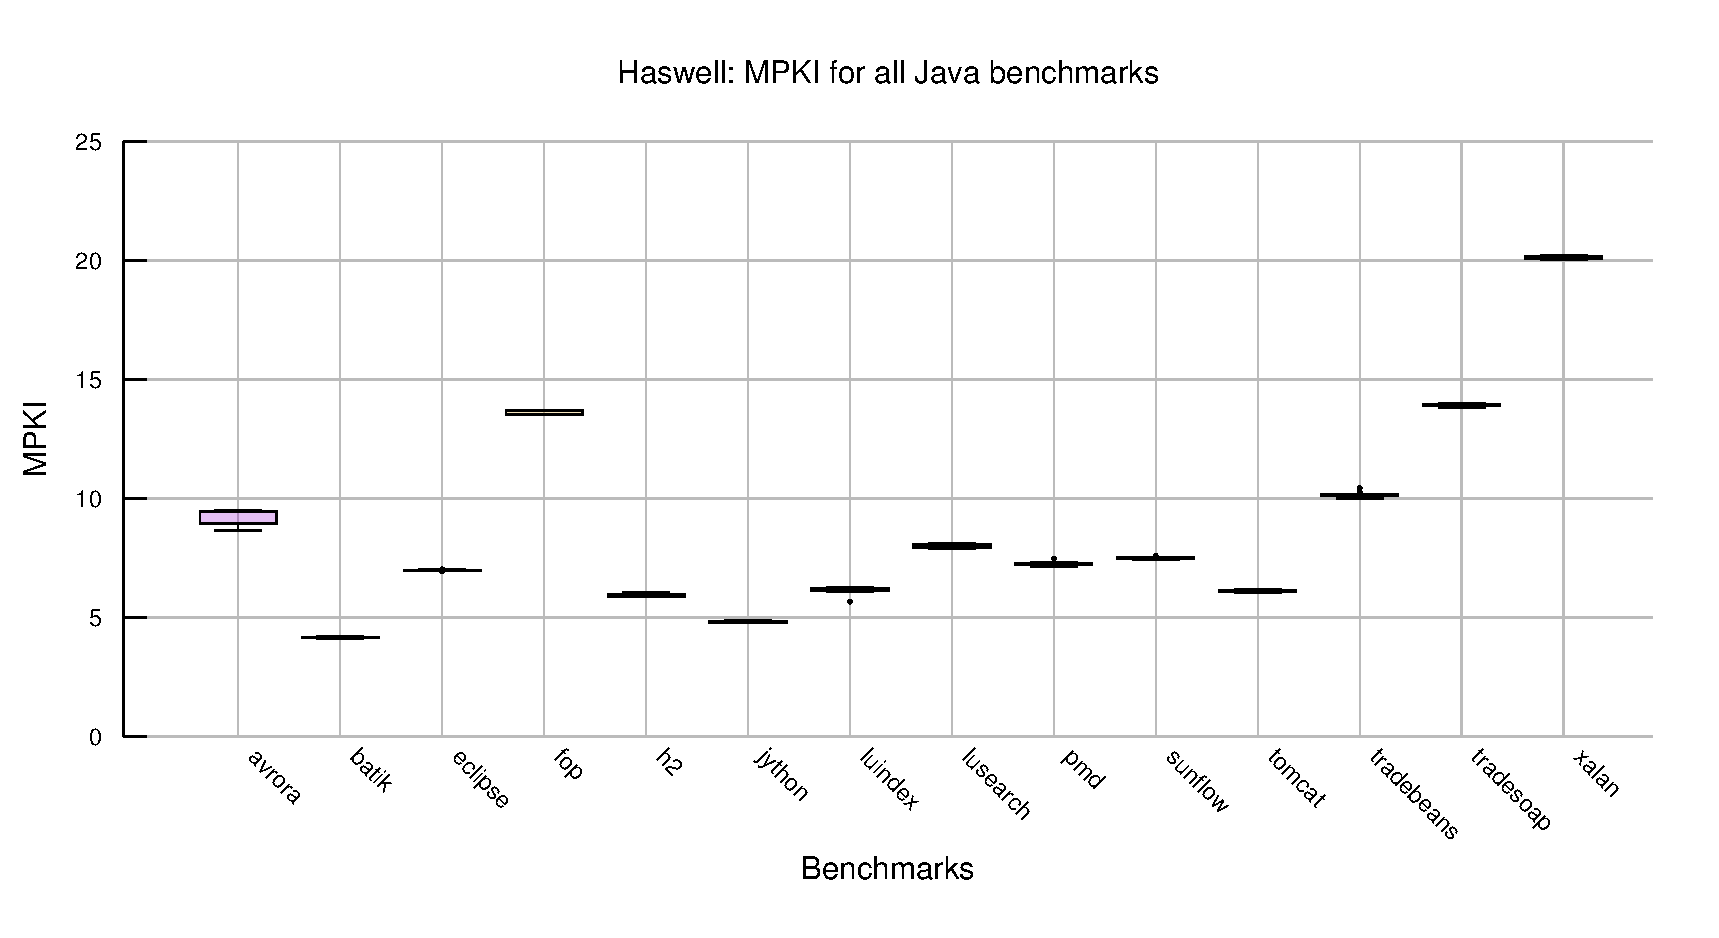
\includegraphics[width=0.5\textwidth]{figures/java_box_haswell.pdf}}
		\subfigure[AMD family15th]
		{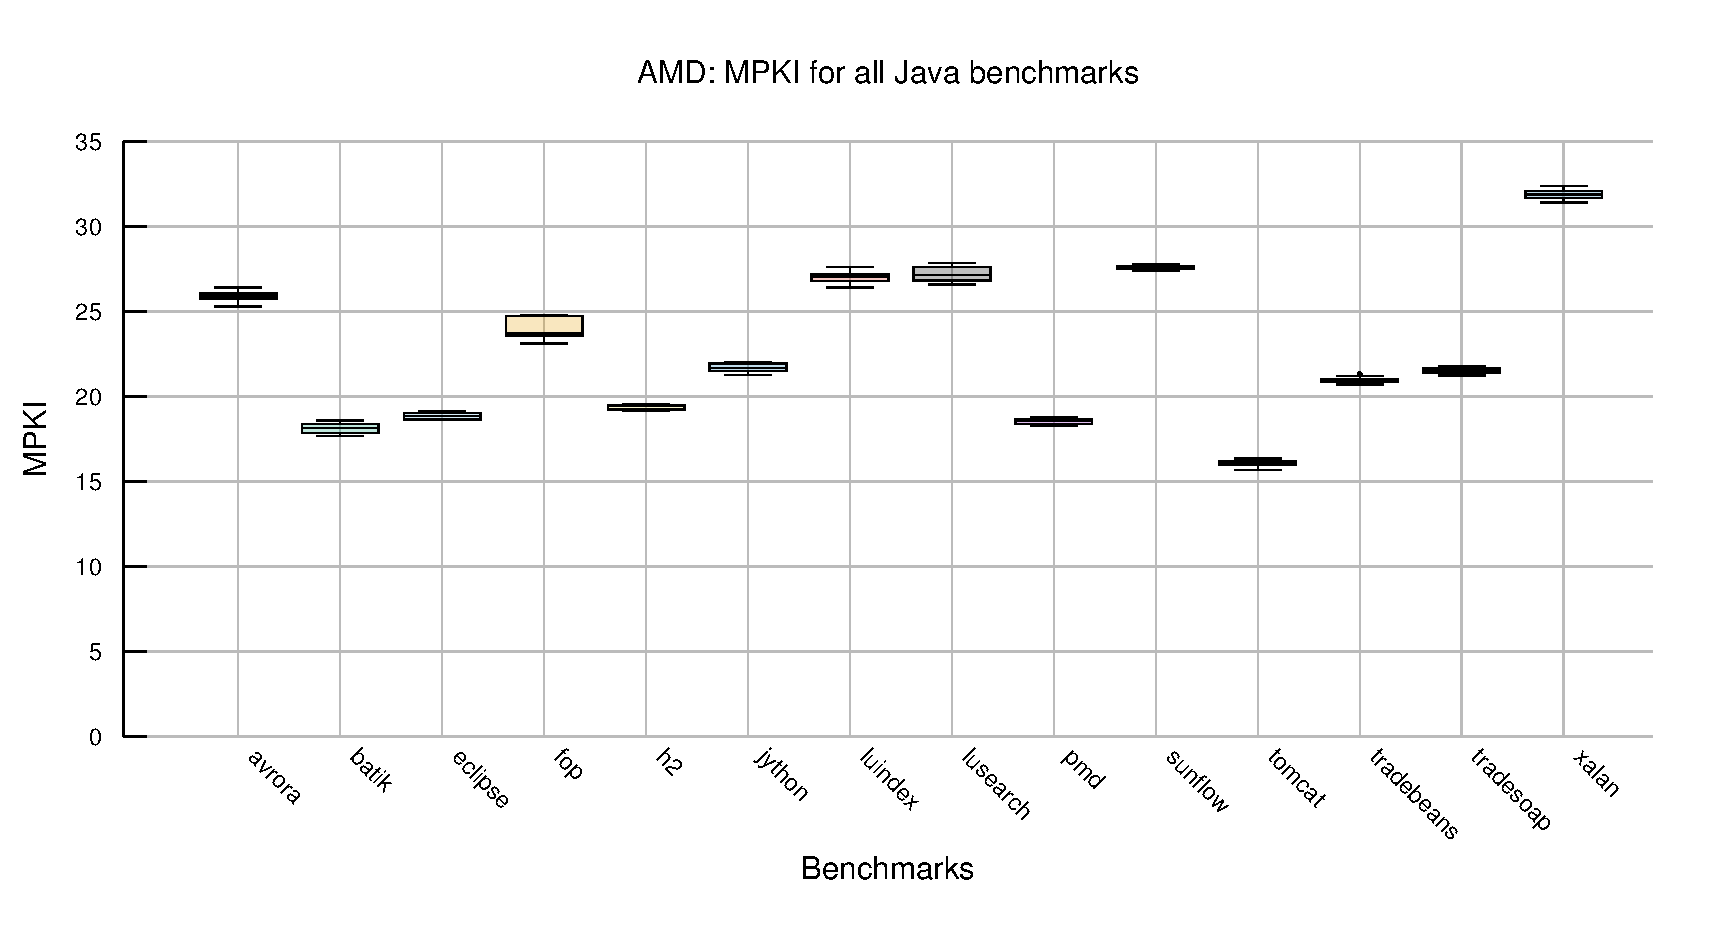
\includegraphics[width=0.5\textwidth]{figures/java_box_amd.pdf}}
		
		\caption{Java: Variation of MPKI for 10 iterations per benchmark for all architectures}
		\label{res:javabox}
	\end{figure*}
	\begin{figure*}[t]
		\subfigure[Core 2 Duo]
		{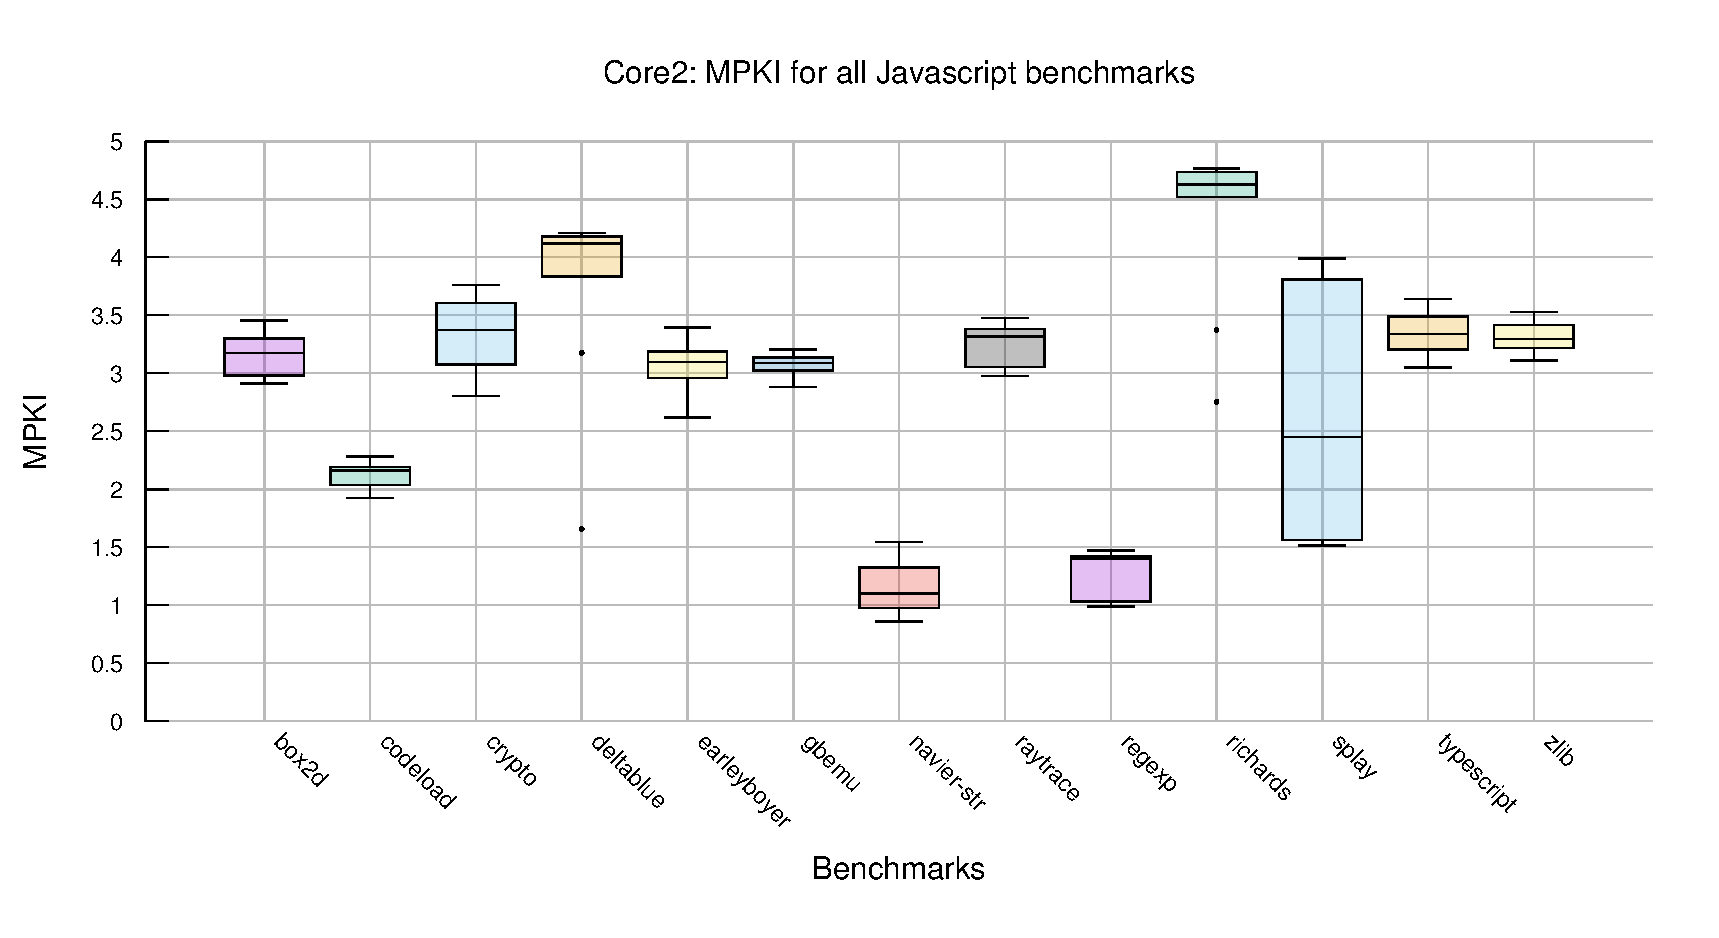
\includegraphics[width=0.5\textwidth]{figures/javascript_box_core2.pdf}}
		\subfigure[Nehalem]%
		{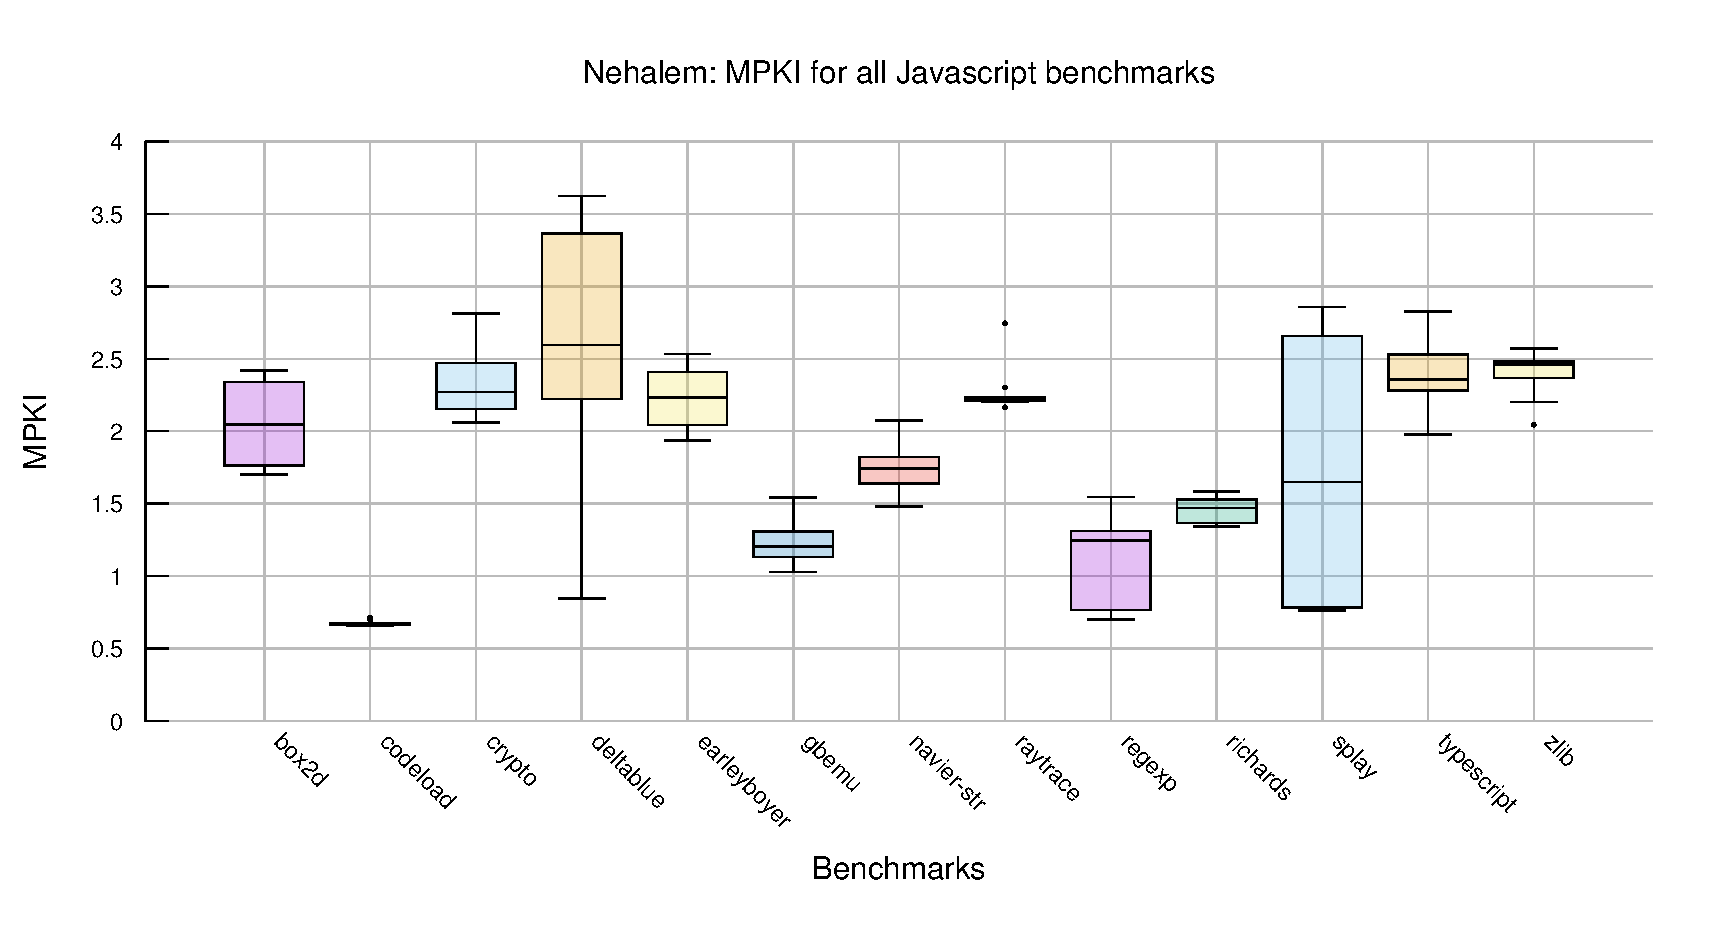
\includegraphics[width=0.5\textwidth]{figures/javascript_box_nehalem.pdf}}
		\subfigure[Ivy Bridge]
		{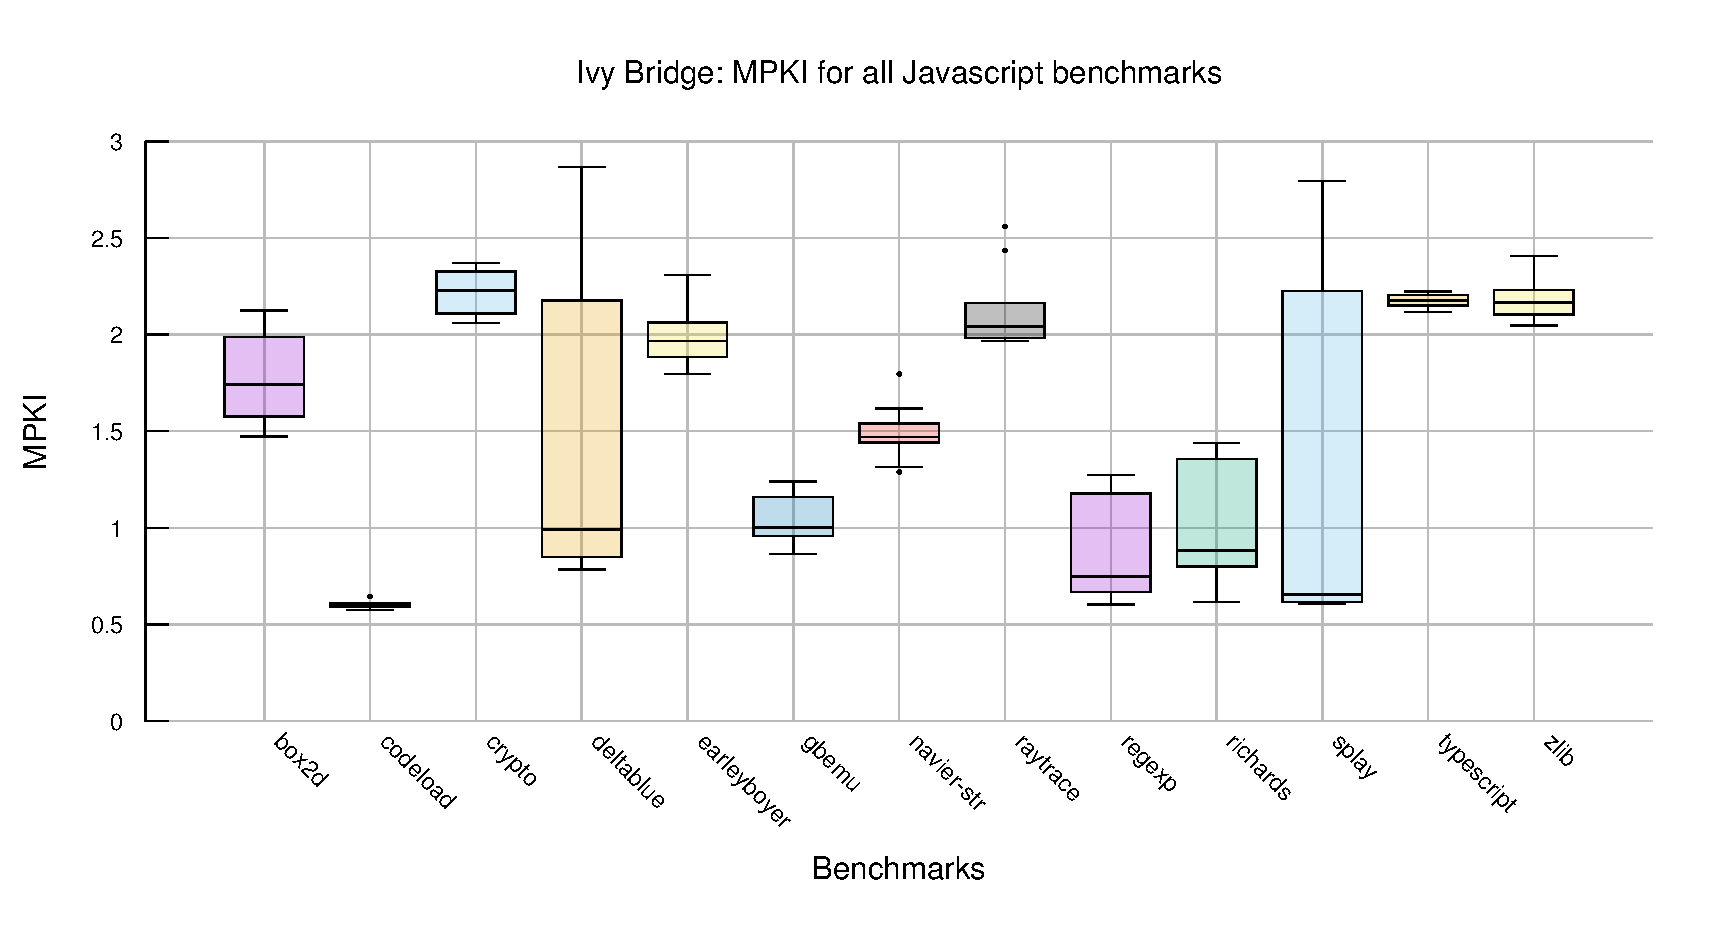
\includegraphics[width=0.5\textwidth]{figures/javascript_box_ivy_bridge.pdf}}	\subfigure[Haswell]
		{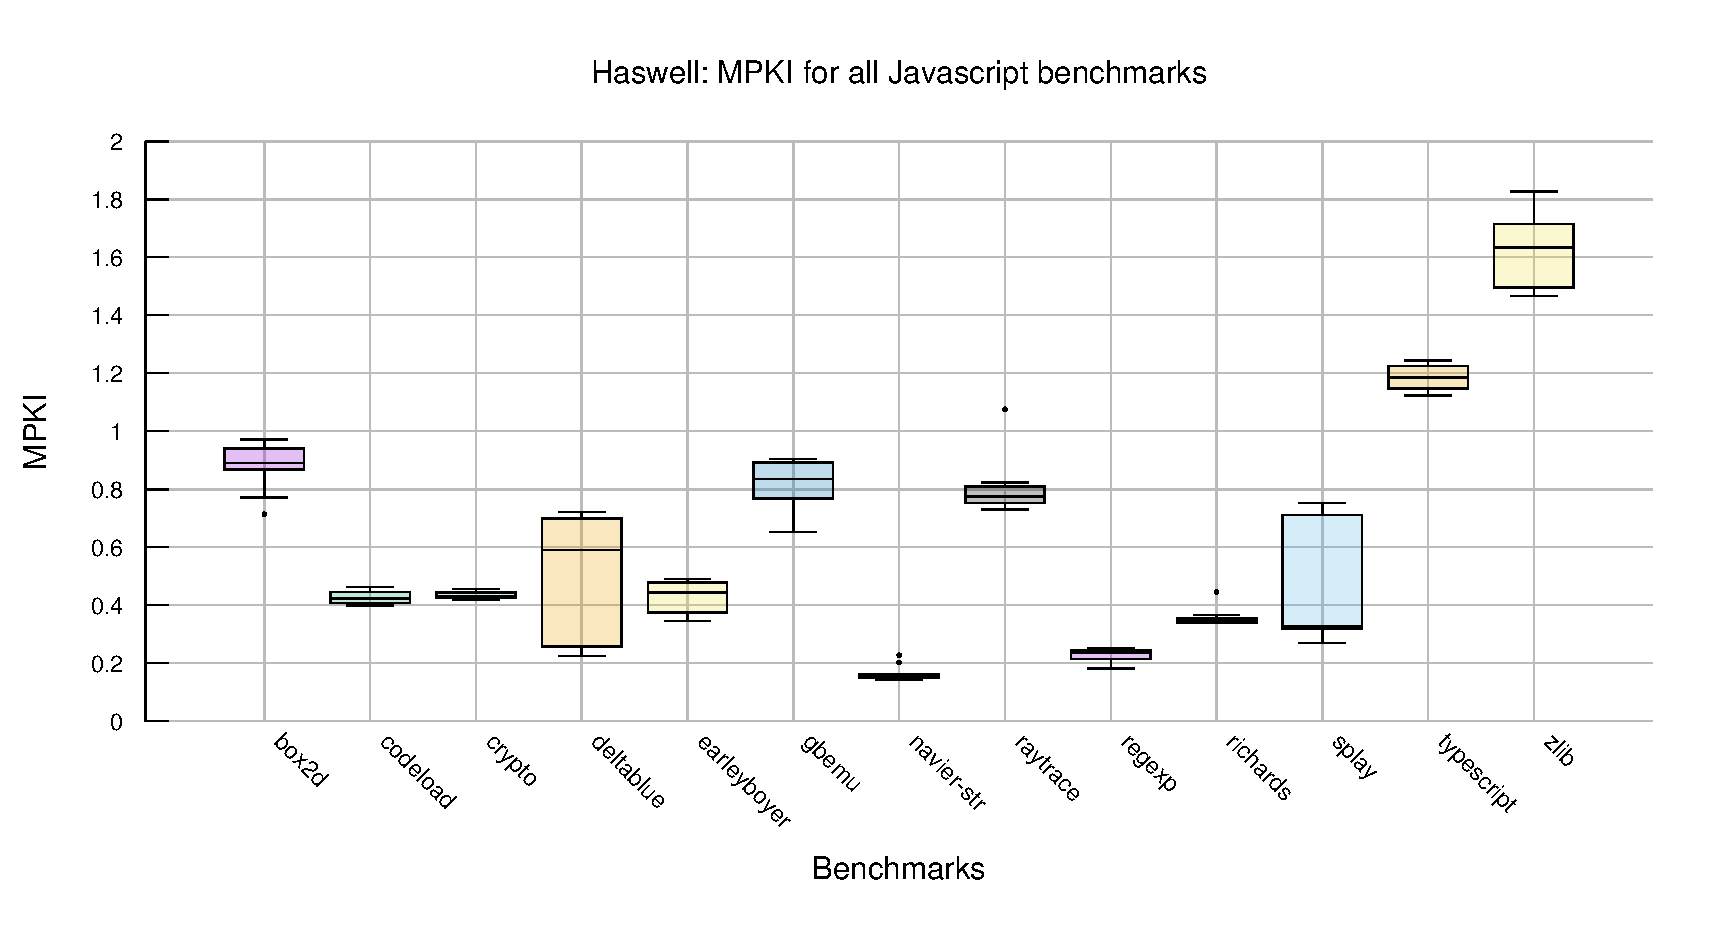
\includegraphics[width=0.5\textwidth]{figures/javascript_box_haswell.pdf}}
		\subfigure[AMD family15th]
		{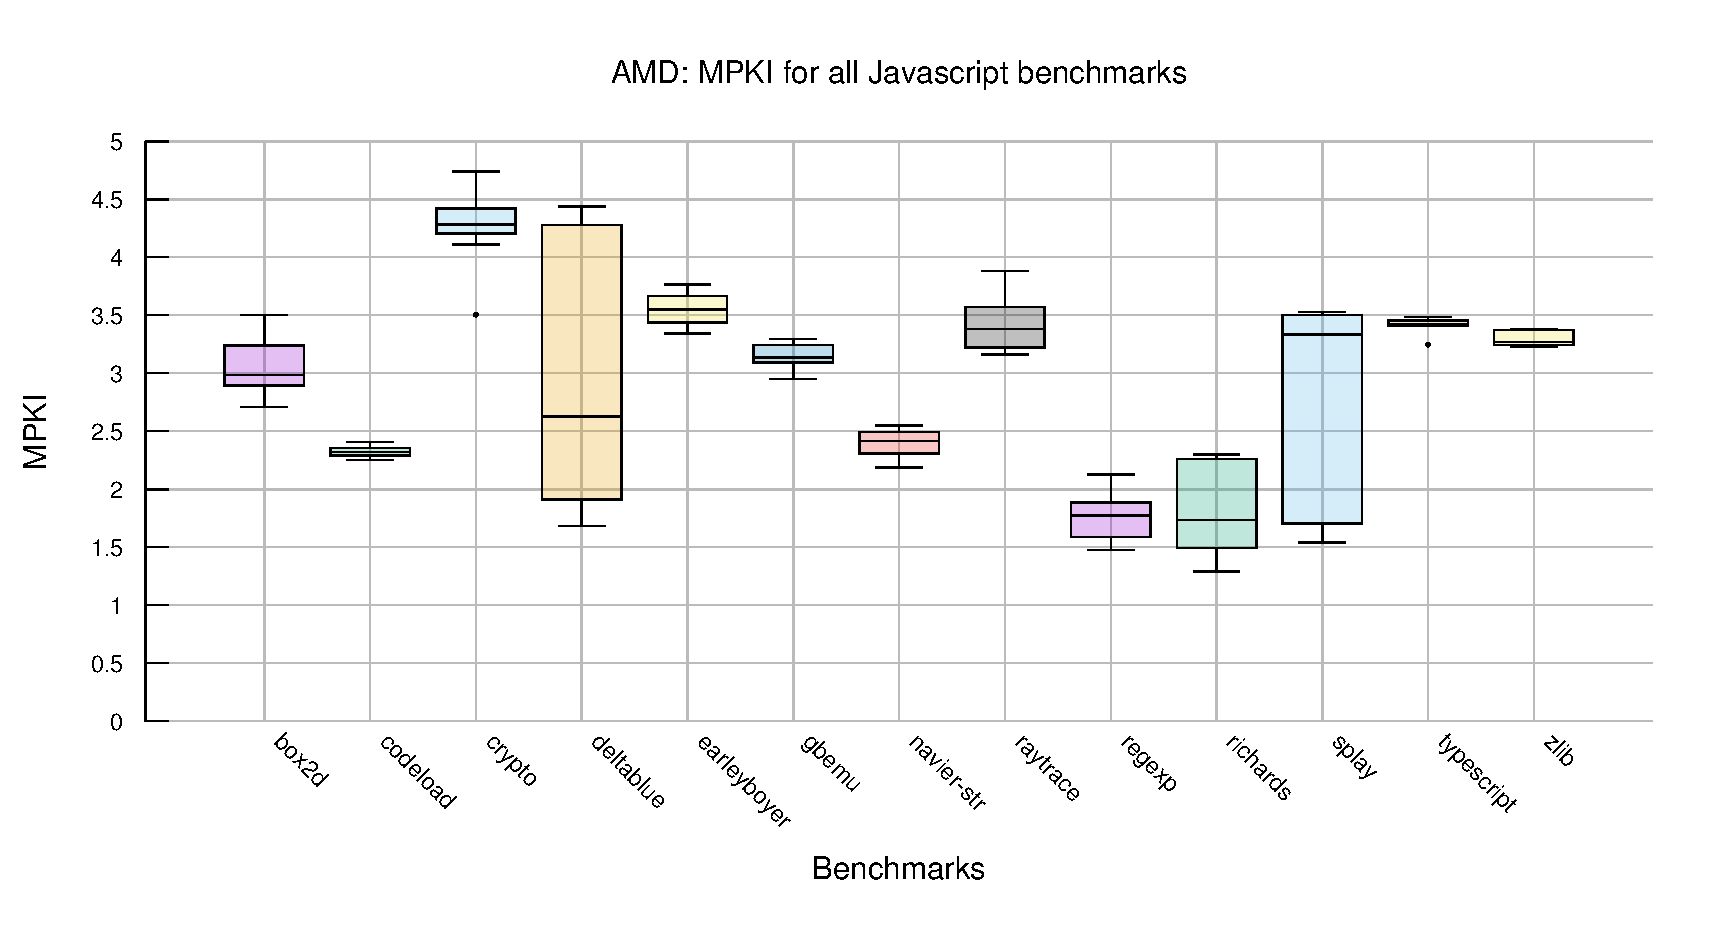
\includegraphics[width=0.5\textwidth]{figures/javascript_box_amd.pdf}}
		
		\caption{Javascript: Variation of MPKI for 10 iterations per benchmark for all architectures}
		\label{res:javascriptbox}
	\end{figure*}
\end{appendices}
\end{document}
